\documentclass[]{standalone}%
%
\usepackage{tikz}%
\usetikzlibrary{angles, calc, patterns, positioning, quotes}%
%
\definecolor{TUMBlack}{cmyk}{0,0,0,1}%
\definecolor{TUMBlue}{cmyk}{1,0.43,0,0}%           Pantone 300
\definecolor{TUMBlue1}{cmyk}{1,0.57,0.12,0.7}%     Pantone 540
\definecolor{TUMBlue2}{cmyk}{1,0.54,0.04,0.19}%    Pantone 301
\definecolor{TUMBlue3}{cmyk}{0.65,0.19,0.01,0.04}% Pantone 542
\definecolor{TUMBlue4}{cmyk}{0.42,0.09,0,0}%       Pantone 283
\definecolor{TUMOrange}{cmyk}{0,0.65,0.95,0}%
\definecolor{TUMGreen}{cmyk}{0.35,0,1,0.2}%
%
\begin{document}%
%
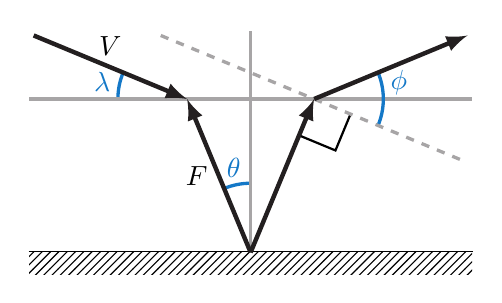
\begin{tikzpicture}[scale = 1]%
    %
    \def\groundheight{.8em}%
    \def\groundwidth{16em}%
    %
    \tikzstyle{arrow} = [->, -latex, ultra thick, draw = TUMBlack]%
    \tikzstyle{dashedline} = [draw = TUMBlack!40, dashed, very thick]%
    \tikzstyle{ground} = [fill = TUMBlack, pattern = north east lines, draw = none, minimum width = \groundwidth, minimum height = \groundheight]%
    \tikzstyle{measurement} = [very thick, draw = TUMBlue, text = TUMBlue, angle eccentricity = 1.25, angle radius = 2.5em]%
    %
    % Ground
    \node (ground) [ground, yshift = -\groundheight/2] {};%
    \draw (ground.north west) -- (ground.north east);%
    %
    \coordinate (origin) at (0, 0);%
    \coordinate [above = 6em of origin, rotate around = {-45/2:(origin)}] (A);%
    \coordinate [above = 6em of origin, rotate around = {45/2:(origin)}] (B);%
    \coordinate [right = 6em of A, rotate around = {45/2:(A)}] (D);%
    \coordinate [right = -6em of B, rotate around = {-45/2:(B)}] (E);%
    \coordinate (F) at ($(A)!6em!270:(origin)$);%
    \coordinate (G) at ($(A)!6em!90:(origin)$);%
    \coordinate (H) at (0, 8em);%
    \coordinate (I) at ($(A)!-5.7em!0:(B)$);%
    \coordinate (J) at ($(B)!-5.7em!0:(A)$);%
    %
    % Angels
    \draw pic [measurement, "$\theta$"] {angle = H--origin--B};%
    \draw pic [measurement, "$\lambda$"] {angle = E--B--J};%
    \pic [draw, thick] {right angle = origin--A--G};%
    %
    % Background
    \draw [very thick, TUMBlack!40] (origin) -- (H);%
    \draw [very thick, TUMBlack!40] (I) -- (J);%
    \draw pic [measurement, "$\phi$"] {angle = I--A--D};%
    \draw pic [measurement] {angle = G--A--I};%
    \draw [dashedline] (F) -- (G);%
    %
    % Force vector
    \draw [arrow] (origin) -- (A);%
    \draw [arrow] (origin) -- (B) node[midway, left] {$F$};%
    %
    % Velocity vector
    \draw [arrow] (A) -- (D);%
    \draw [arrow] (E) -- (B) node[midway, above] {$V$};%
    %
    % Legend
    % \matrix [draw, below left] at (current bounding box.north east) {
    % \node [label = right:force angle $\theta$] {}; \\
    % \node [label = right:velocity angle $\lambda$] {}; \\
    % \node [label = right:collision angle $\phi$] {}; \\
    % };%
    %
\end{tikzpicture}%
%
\end{document}%
%